\glsreset{de}
\glsreset{ea}
\chapter{Der Lösungsansatz}
\label{sec:sol}

	Dieses Kapitel beginnt mit einer Einführung in die Evolutionären Algorithmen und stellt daraus ein Beispiel vor, welches im weiteren Verlauf der Arbeit verwendet wird.

	\section{\gls{ea}}
	\label{sec:evol}
	
		Hierbei handelt es sich, wie in \cite{ea-intro} beschrieben, um heuristische Verfahren zur Lösung von Problemen, die andernfalls nicht in polynomialer Zeit gelöst werden können. Dabei orientieren sie sich an den Vorgängen der biologischen Evolution. Die Begründung hierfür wird von John H. Holland \cite{j-h-holland} in prägnanter Weise dargelegt: 
	
		\begin{quote}
			\textit{Lebewesen sind vollendete Problemlöser. In der Vielzahl der Aufgaben, die sie bewältigen, übertreffen sie die besten Computerprogramme bei weitem - zur besonderen Frustration der Programmierer, die Monate oder gar Jahre harter geistiger Arbeit für einen Algorithmus aufwenden, während Organismen ihre Fähigkeiten durch den scheinbar ziellosen Mechanismus der Evolution erwerben.}
		\end{quote}
	
		Dieses Zitat bietet eine grobe Vorstellung vom Wesen und der Herkunft von \gls{ea}. In vielen literarischen Werken zu diesem Thema - beispielsweise \cite{ger-kla-kru-intro, eib-smi-ea} - wird festgehalten, dass verschiedene Kategorien von \gls{ea}s existieren. Allerdings ist die zugrunde liegende Idee hinter all diesen Sorten von Algorithmen die selbe und wird von den Autoren in \cite{eib-smi-ea} wie folgt dargelegt:\\
		Gegeben sei eine Gruppe von Individuen, genannt \textit{Population}, die innerhalb einer Umgebung mit begrenzten Ressourcen lebt. Der Kampf um diese löst eine natürliche Selektion aus und führt so zu einer höheren Fitness der Population - ein Vorgang, der sehr gut unter dem Stichwort \textit{Survival of the Fittest} bekannt ist. Nach diesem Vorbild aus der Natur nehme man
		\begin{itemize}
			\item ein zu lösendes Problem (stellvertretend für die Umgebung), abgebildet durch eine (Fitness-)Funktion, welche maximiert oder minimiert werden soll, sowie
			\item eine Menge an Lösungskandidaten (im Folgenden als Individuen bezeichnet), bestehend aus einem Set von Funktionsparameterlisten.
		\end{itemize}
		Auf diese Individuen wird sodann die Fitnessfunktion angewendet und mit dem Ergebnis in abstrakter Weise jeweils die Fitness der einzelnen Individuen gemessen. Dabei erfolgt die Bewertung abhängig davon, ob minimiert oder maximiert werden soll. Im folgenden Schritt erzeugen verschiedene Variationsoperatoren wie Mutation und/oder Rekombination aus der Ursprungspopulation eine neue Population, für welche wiederum die Fitnessfunktion ausgewertet wird. Auf der Basis der jeweiligen Fitnesswerte werden die korrespondierenden Individuen beider Populationen verglichen und davon dasjenige mit der höheren Fitness in die Population der nächsten Generation übernommen.
	
		Die oben genannten Schritte werden so lange iteriert, bis entweder eine geeignete Lösung gefunden wurde oder eine (vorher definierte) maximale Anzahl an Iterationen erreicht ist. Abbildung \ref{fig:ea-flowchart}. veranschaulicht die Funktionsweise von \gls{ea}s nochmals in Form eines einfachen Flussdiagramms.
	
		\begin{figure}[h]
			\centering
			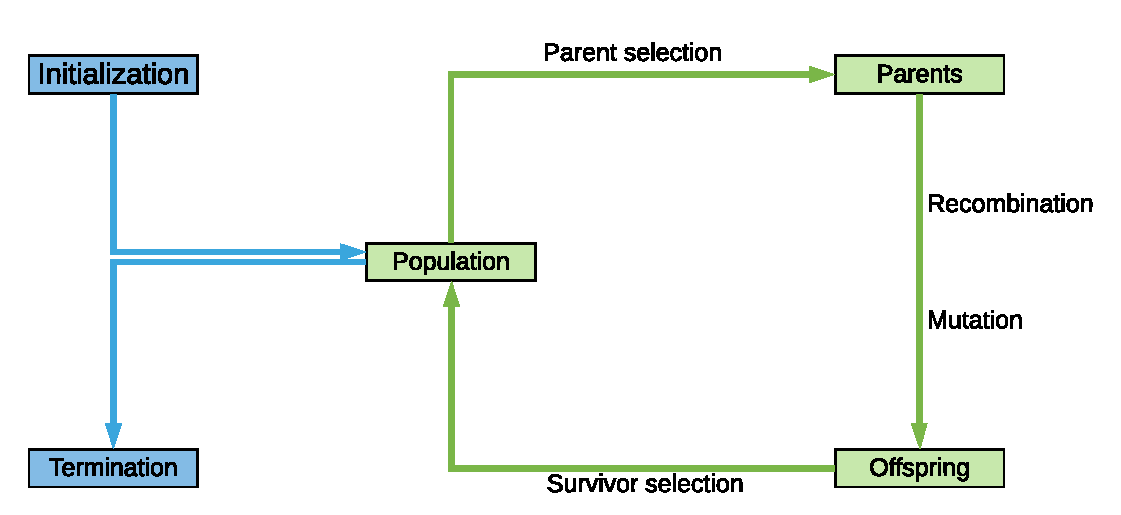
\includegraphics[width=0.7\linewidth]{ea_flowchart}
			\caption[Genereller Ablauf von \gls{ea}s]{Genereller Ablauf von \gls{ea}s (Nachbildung der Graphik aus \cite[Seite 27]{eib-smi-ea})}
			\label{fig:ea-flowchart}
		\end{figure}
	
		Nachstehend wird in Abschnitt \ref{sec:de} der Algorithmus \textit{Differentielle Evolution} als Beispiel aus den \gls{ea} erläutert und in den weiteren Kontext der vorliegenden Arbeit eingebettet.
	
		\glsreset{de}

	\section{\gls{de}}
	\label{sec:de}

		Die Autoren in \cite{storn-price-de} entwickelten den \gls{de}-Algorithmus mit Hinblick auf die im Anschluss gelisteten Anforderungen\footnote{Diese Anforderungen sind zwar in \cite{storn-price-de} lediglich auf Minimierungsprobleme beschränkt, da solche in der Praxis häufiger vorkommen. Allerdings sind sie auf Maximierungsprobleme ebenso anwendbar.}
		an eine in der Praxis anwendbare Optimierungsmethode:
		\begin{enumerate}
			\item Sie soll mit nicht-differenzierbaren und nicht-linearen 
			Funktionen, welche unter Umständen mehrere (lokale) Maxima/Minima 
			aufweisen, umgehen können.
			\item Falls eine sehr rechenintensive Funktion auftritt, soll die Optimierungsmethode parallelisierbar sein. Es soll also möglich sein, die Berechnungen auf mehrere Prozessorkerne auszulagern.
			\item Weiterhin soll die Optimierungsmethode leicht zu benutzen sein. Im gegebenen Kontext bedeutet dies zum Beispiel, dass sie wenige Kontrollparameter besitzt, die einfach bestimmbar sind.
			\item Außerdem soll sie sich mit steigender Iterationszahl immer 
			näher dem \textbf{globalen} Minimum/Maximum annähern.
		\end{enumerate}
		
		Die ursprüngliche Variante \gls{de}1 ist hierbei folgendermaßen beschrieben:\\
		Den Ausgangspunkt, wie in Abschnitt \ref{sec:evol} bereits erläutert, bildet eine Population aus $N_{P}$ Individuen $x_{i, G}$, wobei $N_{p}$ die Populationsgröße, $i$ der Populationsindex und $G$ der Generationsindex ist. 